%%%%%%%%%%%%%%%%%%%%%%% file template.tex %%%%%%%%%%%%%%%%%%%%%%%%%
%
% This is a general template file for the LaTeX package SVJour3
% for Springer journals.          Springer Heidelberg 2010/09/16
%
% Copy it to a new file with a new name and use it as the basis
% for your article. Delete % signs as needed.
%
% This template includes a few options for different layouts and
% content for various journals. Please consult a previous issue of
% your journal as needed.
%
%%%%%%%%%%%%%%%%%%%%%%%%%%%%%%%%%%%%%%%%%%%%%%%%%%%%%%%%%%%%%%%%%%%
%
% First comes an example EPS file -- just ignore it and
% proceed on the \documentclass line
% your LaTeX will extract the file if required
%
\RequirePackage{fix-cm}
%
%\documentclass{svjour3}                     % onecolumn (standard format)
%\documentclass[smallcondensed]{svjour3}     % onecolumn (ditto)
\documentclass[smallextended]{svjour3}       % onecolumn (second format)
%\documentclass[twocolumn]{svjour3}          % twocolumn
%
\smartqed  % flush right qed marks, e.g. at end of proof
%\usepackage{cite}
\usepackage{amsmath, amssymb, amsfonts}
%\usepackage{algorithmic}
\usepackage{graphicx}
\usepackage{enumitem}
\usepackage[misc]{ifsym}
\usepackage{tabularx}
\usepackage{booktabs}

%\usepackage{titling}
%\thanks{}
%\usepackage{textcomp}
%\usepackage{indentfirst}
%\usepackage{amsthm}
%\usepackage[marginal]{footmisc}
\allowdisplaybreaks[4]
%\newcommand*{\affaddr}[1]{#1} % No op here. Customize it for different styles.
%\newcommand*{\affmark}[1][*]{\textsuperscript{#1}}
%\newtheorem{theorem}{Theorem}  
%\newtheorem{lemma}{Lemma}
%\newtheorem{remark}{Remark}
%\newtheorem{correctness}{Correctness}
%
% \usepackage{mathptmx}      % use Times fonts if available on your TeX system
%
% insert here the call for the packages your document requires
%\usepackage{latexsym}
% etc.
%
% please place your own definitions here and don't use \def but
% \newcommand{}{}
%
% Insert the name of "your journal" with
% \journalname{myjournal}
%

%\smartqed

%\AtBeginDocument{%
%  \setlength{\oddsidemargin}{\dimexpr(\paperwidth-\textwidth)/2-1in}%
%  \setlength{\evensidemargin}{\oddsidemargin}%
%  \setlength{\topmargin}{%
%    \dimexpr(\paperheight-\textheight)/2-\headheight-\headsep-1in}%
%}

\begin{document}

% \title{An Efficient CP-ABE with Privacy-preserving and Decryption Testing Scheme in Cloud Computing}
\title{A Verifiable Hidden Tree Structure CP-ABE with Decryption Testing Scheme and its Application in Cloud Computing}
%\titlerunning{Short form of title}        % if too long for running head


\author{ 
	Yang  Zhao \and %\affmark[1]\and 
	Hu Xiong 
}
\clearpage


%\authorrunning{Short form of author list} % if too long for running head

\institute{ Yang Zhao \at
University of Electronic Science and Technology of China, Chengdu, 610054 , China.\\
\email{zhaoyang@uestc.edu.cn}
\and
\Letter \   Hu Xiong  \at
University of Electronic Science and Technology of China, Chengdu, 610054 , China.\\
Guangxi Colleges and Universities Key Laboratory of cloud computing and complex systems, Guilin University of Electronic Technology, Guilin, 541004, China.\\
\email{xionghu.uestc@gmail.com} \\
%\affaddr{\affmark[1] University of Electronic Science and Technology of China, Chengdu , China.}
}

\date{Received: date / Accepted: date}
% The correct dates will be entered by the editor

\maketitle

\begin{abstract}
	% With the rapid increase of data and the tremendous improvement of cloud computing infrastructures, more and more users are storing their personal data(e.g electronic medical records, address books, smart phone data etc.) in cloud, but the security of cloud storage supported by cloud service providers(CSP) is semi-secure to users, and the privacy of users cannot be fully guaranteed. 
	% Therefore, how to protect the security and confidentiality of data in cloud storage has become hot spot that researchers pay attention to. 
	% Since attribute-based encryption has the characteristics of one-to-many encryption and fine-grained access control, attribute-based encryption scheme is widely considered as an ideal solution. 
	% However, the basic CP-ABE encryption scheme has the flaws that access structure may leak user privacy, inefficiency, and weak expression ability. 
	% In view of the above shortcomings, this paper proposes a CP-ABE encryption scheme with the following features: 
	% 1. in order to enhance the express ability the access structure, we adopt a tree-based access structure instead of the widespread AND gate structure; 
	% 2. a testing phase is used to eliminate unnecessary operations and improve decryption efficiency; 
	% 3. to fully utilize the resources of the cloud server and decrease the local decryption options, we outsource the time-consuming pairing operation to security cloud server. 
	% Besides, the scheme is provably secure against adaptively chosen-ciphertext attack. 
	% Finally, we apply our scheme into EMR system established in cloud computing environment.
	Ciphertext policy attribute based encryption(CP-ABE) is widely used in secure data sharing with one-to-many feature and the characteristics of fine-grained access. 
	However, the basic CP-ABE encryption scheme has the flaws that access structure may leak user privacy.
	At the same time, excessive bilinear pairing operations in decryption phase are a significant burden for users participating in the system. 
	Furthermore, the verifiable decryption testing is not explored in CP-ABE.
	Based on the above three factors, we propose a verifiable hidden tree structure CP-ABE with decryption testing scheme in this paper.
	Besides, the scheme is provably secure against adaptively chosen-ciphertext attack. 
	Finally, we apply our scheme into EMR system established in cloud computing environment.
\keywords{CP-ABE;hidden policy;verifiable decryption testing;cloud computing}
\end{abstract}

\section{Introduction}
	In the era of data explosion, with the tremendous improvement of cloud computing infrastructures, cloud computing platforms have given users a better and more convenient way to share data and store data.
	%Users can store and retrieve their own data on the cloud platform and also easily share data with other users on the cloud platform. 
	However, since the user stores the data on the cloud platform and the data is out of the user's control, it will bring out many severe issues.
	One of the most obvious problem is if malicious users attack cloud server and obtain the data belonging to normal users, the user's privacy will be leaked and even causes incalculable losses. 
	Therefore, how to ensure the privacy of users and the security of cloud data sharing has become an urgent problem to be solved. 
	ABE as a novel encryption notation, not only provides access control but also provides the function of encrypting data, consequently, it is regarded as a promising method to handle this matter. 
	Although attribute-based encryption can solve above problems, it has another hidden danger which is access structure is passed in plaintext during the process of encryption and decryption.
	Once some malicious attackers steal the access structure stored in clear text, the user's privacy will also be revealed. 
	Thus, it is crucial to encrypt the access structure.

	Here we take the EMR system as an example. 
	Figure\ref{EMR1} is a simple Electronic Medical Record System structure. 
	For convenience, we simplify EMR system to three parts: data owner(including patients), cloud storage server(CSS), data recipient(including doctor, malicious attacker).
	The data owner encrypt his EHR via CP-ABE and upload it to CSS. 
	CSS are deployed in an open environment that anyone can access.
	Under normal circumstances, a data recipient who has the private key can decrypt ciphertext and obtain EMR transmitted by data owner.
	For example, both doctorA and doctorB in Figure\ref{EMR1} can normally decrypt the EMR because their private keys satisfy access structure.
	In another case, for a malicious attacker, although he can not decrypt the EMR, he is able to get the access structure stored in plaintext and obtain the data owner's information.
	For instance, in Figure\ref{EMR1}, the malicious may get the sensitive information that patient whose $PID$ is 28496 suffers from diabetes.  


	\begin{figure}\label{EMR1}
		\centering
		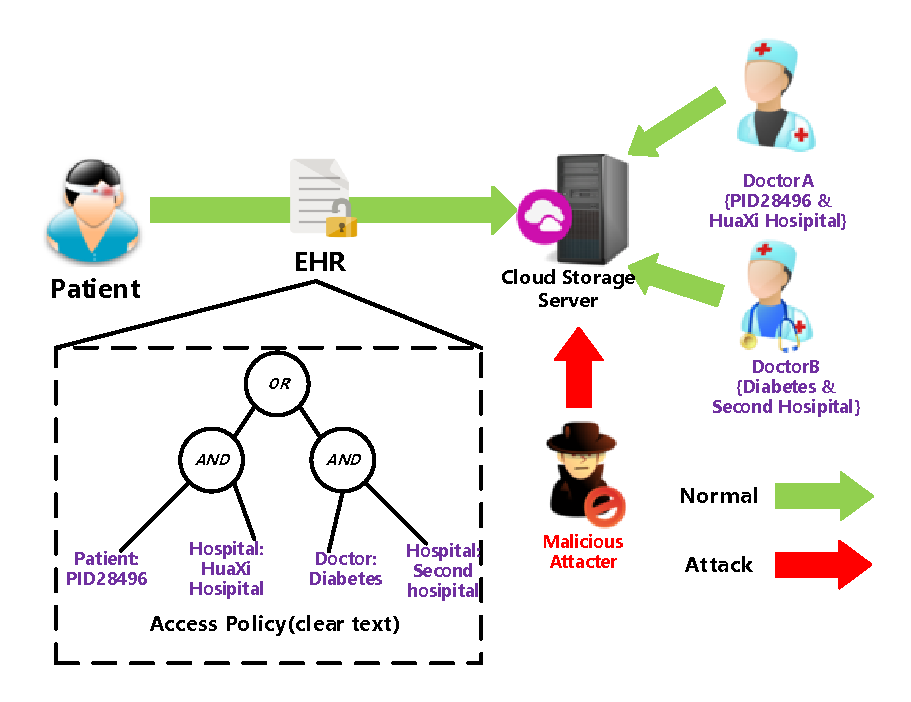
\includegraphics[width=3.8in, keepaspectratio]{EMR1.pdf}
		\caption{EMR Structure}
	\end{figure}
 
\subsection{Related Work}
	Since Shamir introduced the idea of identity-based encryption(IBE) to address certificate management and update issues in public key cryptography, Sahai and Waters proposed a fuzzy identity-based encryption scheme(Fuzzy IBE) based on IBE. 
	% In the scheme, the user's identity is used as the public key, and the public key is allowed to be an arbitrary string, such as an email address.
	% However, IBE can only achieve one-to-one decryption, which means that the owner encrypts the message through the recipient's public key, and the message can only be decrypted by the receiver, which is coarse-grained access control. 
	In the Fuzzy IBE, the user has multiple identity attributes, and only the decryptor needs to satisfy the threshold $d$ identity features to decrypt correctly. 
	This is the original Attribute-Based Encryption(ABE) mechanism. 
	Afterwards there were two kinds of schemes derived from it, key policy attribute based encryption(KP-ABE) and ciphertext policy attribute based encryption(CP-ABE). 
	Compared to KP-ABE, CP-ABE could be deployed in more schemes and applications for the more flexible. 
	Therefore, we mainly discuss different CP-ABE schemes in the rest of this paper.

	% a new paragraph
	Currently, there are three types of access structures that are utilized in proposed CP-ABE schemes, AND gate, tree structure and linear secret sharing scheme(LSSS).
	[][][][][][][][][][][][][][][][].

	% a new paragraph
	Different access structures can only improve the expressive ability, and can not solve the problem of the access structure leaking user privacy.
	In 2008, Nishide et al. proposed a partially hidden CP-ABE scheme to overcome the above problems. 
	They used AND gate on multi-valued attributes with wildcard access structures and used inner product predicate encryption techniques, and proved that their scheme is selectively secure. 
	In 2011, Lai et al. improved the Nishide et al. scheme and proposed a fully secure hidden policy scheme with the same access structure used in Nishide et al. 
	The problem with this approach is that the size of the ciphertext grows with the number of attributes and leads to higher computational costs. 
	In 2012, Li et al. used dual-system cryptography to achieve a completely secure access structure hiding scheme over a composite order group. 
	In 2013, Hur proposed an attribute-based encryption scheme for hidden policy of the smart grid. 
	Under the premise of hiding the access structure, a scheme for implementing arbitrary monotonic expressions is presented. 
	But the weak points are that the user has a long length of secret key in the scheme, and no security proof is given. 
	In 2015, Xu et al. proposed a CP-ABE scheme that supports access structure hiding based on the tree access structure, which further improved the expressiveness of the access strategy but efficiency is the bottleneck of the scheme. 
	In 2015, Yadav et al. gave three states for each attribute in the access structure and calculated its corresponding user secret key and ciphertext to achieve a fully hidden access policy. 
	However, the scheme only supports "AND" gate, and the expression ability is relatively weak. 
	In 2016, Phuong et al. proposed a new scheme to overcome the ciphertext size problem in hidden strategies. 
	However, the cumbersome user private key calculation process and complex encryption and decryption operations limit its application.

	% a new paragraph
	For most CP-ABE schemes, complex pairing operations result in low efficiency, further, it limits the practical application of these schemes.
	Green et al. firstly introduced the notion of ABE with outsourced decryption to solve the issue of low efficiency. 
	Afterwards, Lai et.al optimized Green's scheme and added verification function to guarantee the correctness of the transformation done by the cloud server.
	It perfectly settles the issues including low efficiency and correctness of transformation ciphertext, while there are parallel instances in the encryption and decryption algorithms, it can increase communication overhead.
	Lin et al. used key derivation function(KDF) and random function techniques to successfully reduce excessive communication overhead.
	

	% a new paragraph
	Through the CP-ABE encryption scheme mentioned above, we can find that although they all have the identical function of hidden policy, there is a problem that cannot be neglected in terms of efficiency. 
	The efficiency of scheme is a key points we have to consider when scheme is applied in actual scene. 
	Moreover, most of the schemes use the access structure with AND gate, which cannot indicate threshold value, and the expression ability is lower compared with the LSSS and the tree-based structure. 
	Finally, as mentioned above, due to the limitation of efficiency, most of the solutions do not propose a reasonable application scenario.

\subsection{Our Contribution}
	User privacy-preserving and the efficiency of the solution prompt us to propose a new CP-ABE solution. %called CP-ABE-HPT. 
	In order to balance expression ability of access structure, we adopted a tree-based access structure in terms of policy hiding. 
	For the computational complexity of the pairing operation, we make reasonable use of the advantages of cloud computing, outsourcing the decryption operation to the cloud computing server with stronger computing performance, so as to reduce the user's local calculation. 
	In addition, during the outsourcing calculation phase, we added an additional testing step (see the implementation section for details) to further reduce the amount of calculation. 
	As numerous previous schemes, we also provide the proof which indicates the scheme meets Chosen Ciphertext Attack(CCA) security of the security of our scheme. 
	Further, we depicted an EMR system architecture and smoothly embedded our solution in it. 
	Ultimately, we demonstrate the efficiency of our scheme from both theoretical analysis and simulation experiments.

\subsection{Organization}
	The remainder of this article consists of the followings. 
	In section\ref{section2}, we list some preliminaries that are used in our scheme. 
	Then, the concrete scheme and an EMR system are entirely demonstrated in section\ref{section3}. 
	Section\ref{section4} proposes the security proof of our scheme. Finally, in section\ref{section5}, the performance analysis of our scheme is illustrated.


\section{Preliminaries}\label{section2}
\subsection{Access Structure}
	The same access structure as [\ref{}] we adopt. 
	Let ${P_1,P_2,...,P_n}$ be a set of parties.
	A collection $\mathbb{A}\subseteq 2^{\{P_1,P_2,...,P_n\}}$ is monotone if $\forall B,C:$ if $B\in \mathbb{A}$ and $B \subseteq C$ then $C \in \mathbb{A}$.
	An access structure (respectively, monotone access structure) is a collection(respectively, monotone collection) $\mathbb{A}$ of non-empty subsets of $\{P_1,P_2,...,P_n\}$, i.e., $\mathbb{A} \subseteq 2^{\{P_1,P_2,...,P_n\}}\setminus\{\varnothing \}$.
	The sets in $\mathbb{A}$ are called the authorized sets, and the sets not in $\mathbb{A}$ are called the unauthorized sets.

	In our scheme, the $P_i$ are replaced by attributes.
	We define the collection $\mathbb{A}=\{a_1,a_2,..,a_n\}$ contains all of the authorized attributes in system where $n$ is the number of authorized attributes. 
	For $\forall i \in \mathbb{Z}_N$, the value set of attribute $a_i$ is $\mathbb{V}_i=\{v_{i,1},v_{i,2},...,v_{i,n_i}\}$, similarly, $n_i$ is the amount of elements of $\mathbb{V}_i$.
	The collection $\mathbb{L}=\{l_1=v_{1,t_1},l_2=v_{2,t_2},...,l_k=v_{k,t_k}\}$ is a subset of system attributes set $\mathbb{A}$ and it is used to denote the collection of user attributes where $k$ is the number of user attributes.  

\subsection{Composite Order Bilinear Groups}
	This paper utilizes a bilinear group with a product of three unique prime numbers. 
	Assume that the group generation algorithm $\mathcal{G}$ has a security input parameter $1^{\lambda}$ and it outputs a tuple $(p,q,r,\mathbb{G},\mathbb{G}_{T},e)$ where $p,q,r$ are distinct primes($p,q,r>2^{\lambda}$), $\mathbb{G}$ and $\mathbb{G}_{T}$ are cyclic groups of order 
	$N=pqr$. $\mathbb{G}_{p},\mathbb{G}_{q},\mathbb{G}_{r}$ 
	whose order are ${p,q,r}$ separately are the subgroups of group $\mathbb{G}$. 
	The $e:\mathbb{G}\times\mathbb{G}\to\mathbb{G}_{T}$ is a map with the following requirements:
\begin{itemize}
	\item[$\bullet$] Bilinear: $\forall g,h \in \mathbb{G}, \forall a,b \in \mathbb{Z}_{N},e(g^a,h^b)=e(g,h)^{ab};$
	\item[$\bullet$] Non-degenerate: $\exists g \in \mathbb{G}$ such that $e(g,g)$ has the order $N$ in $\mathbb{G}_{T}$;
	\item[$\bullet$] Computable: $\mathbb{G}$ and $\mathbb{G}_{T}$ are bilinear groups if the group operations in  $\mathbb{G},\mathbb{G}_{T}$ and the bilinear map $e:\mathbb{G}\times\mathbb{G}\to\mathbb{G}_{T}$ are both computable in polynomial time.
\end{itemize}
	We use $\mathbb{G}_p$ and $\mathbb{G}_q$ to denote the subgroups of $\mathbb{G}$ with order $p$ and $q$ respectively. Note that the following two properties:
\begin{itemize}
	\item [1).] $\forall h_p \in \mathbb{G}_p, \forall h_q \in \mathbb{G}_q, e(h_p,h_q)=1$;
	\item [2).] $\forall h_p \in \mathbb{G}_p, \forall h_q \in \mathbb{G}_q, \forall a,b,c,d \in \mathbb{Z}_N,$\\ $e(h_{p}^{a}h_{q}^{b},h_{p}^{c}h_{q}^{d})=e(h_p,h_q)^{ab}=e(h_p,h_q)^{cd}$.
\end{itemize}

\subsection{Complexity Assumptions} \label{Complexity_Assumptions}
	Now we cite the complexity assumptions we use in this paper. 
	The assumption is just the subgroup decision problem in the case where the group order is the product of three prime orders.
	Note that the assumptions have two characteristics, non-interactive and fixed size like in \ref{}.  
	Let $\mathbb{G}_{pq}$ indicates the subgroup with order $pq$.
%Assumption environment%
\newtheorem{myAssumption}{Assumption} 
%Definition environment%
\newtheorem{myDefinition}{Definition}
%Assumption1%
\begin{myAssumption}\label{myAssumption1}
	We define the following distributions: \\
	$\mathbb{G}=(N=pqr,\mathbb{G},\mathbb{G}_T,e)\leftarrow\mathcal{G}(1^{\lambda}),g_p\stackrel{R}{\longleftarrow}\mathbb{G}_p,g_r\stackrel{R}{\longleftarrow}\mathbb{G}_r,D=(\mathbb{G},g_p,g_r),$\\
	$T_1\stackrel{R}{\longleftarrow}\mathbb{G}_{pq},T_2\stackrel{R}{\longleftarrow}\mathbb{G}_p$
\end{myAssumption} 
%Definition1%
\begin{myDefinition}
	\item We define the advantage of algorithm $\mathcal{A}$ to break Assumption1 as: $Adv_{g,\mathcal{A}(\lambda)}^{1}=|Pr[\mathcal{A}(D,T_1)=1]-Pr[\mathcal{A}(D,T_2)=1]|$.
\end{myDefinition}

%Assumption2%
\begin{myAssumption}\label{myAssumption2}
	We define the following distributions:\\
	$\mathbb{G}=(N=pqr,\mathbb{G},\mathbb{G}_T,e)\leftarrow\mathcal{G}(1^{\lambda}),g_p, X_1\stackrel{R}{\longleftarrow}\mathbb{G}_p, X_2\stackrel{R}{\longleftarrow}\mathbb{G}_q,g_r\stackrel{R}{\longleftarrow}\mathbb{G}_r,D=(\mathbb{G},g_p,g_r,X_1,X_2),$\\
	$T_1\stackrel{R}{\longleftarrow}\mathbb{G}_{pq},T_2\stackrel{R}{\longleftarrow}\mathbb{G}_p$
\end{myAssumption} 
% Definition2
\begin{myDefinition}
	\item We define the advantage of algorithm $\mathcal{A}$ to break Assumption2 as: $Adv_{g,\mathcal{A}(\lambda)}^{2}=|Pr[\mathcal{A}(D,T_1)=1]-Pr[\mathcal{A}(D,T_2)=1]|$.
\end{myDefinition}

%Assumption3%
\begin{myAssumption}\label{myAssumption3}
	We define the following distributions: \\
	$\mathbb{G}=(N=pqr,\mathbb{G},\mathbb{G}_T,e)\leftarrow\mathcal{G}(1^{\lambda}),\omega,s \in \mathbb{Z}_N, g_p\stackrel{R}{\longleftarrow}\mathbb{G}_p, X_2, Y, Z_2\stackrel{R}{\longleftarrow}\mathbb{G}_q,g_r\stackrel{R}{\longleftarrow}\mathbb{G}_r,D=(\mathbb{G},g_p,g_p^{\omega}X_2,g_p^{s}Y_2,Z_1Z_2,g_r),$\\
	$T_1\stackrel{R}{\longleftarrow}e(g_p,g_p)^{\omega s},T_2\stackrel{R}{\longleftarrow}\mathbb{G}_p$
\end{myAssumption} 
% Definition3
\begin{myDefinition}
	\item We define the advantage of algorithm $\mathcal{A}$ to break Assumption3 as: $Adv_{g,\mathcal{A}(\lambda)}^{3}=|Pr[\mathcal{A}(D,T_1)=1]-Pr[\mathcal{A}(D,T_2)=1]|$.
\end{myDefinition}
\begin{myDefinition}
	If algorithm $\mathcal{A},Adv_{g,\mathcal{A}(\lambda)}^{1},Adv_{g,\mathcal{A}(\lambda)}^{2},Adv_{g,\mathcal{A}(\lambda)}^{3}$ can be ignored in any polynomial time, the $\mathcal{G}$ will satisfy Assumption1$\sim$3. 
\end{myDefinition}

\subsection{Security Model}
We will give a adaptively-CCA security model for our scheme. 
The security game between adversary $\mathcal{A}$ and  Challenger $\mathcal{C}$ is described as followings:
\begin{itemize}
	\item \textbf{Setup: }The challenger $\mathcal{C}$ runs initialization algorithm $Setup(1^\lambda)$ to generates public key $PK$ and master secret key $MSK$. Then $\mathcal{C}$ stores $MSK$ and transfers $PK$ to $\mathcal{A}$.
	\item \textbf{Phase1: }$\mathcal{A}$ asks $\mathcal{C}$ secret key of attribute sets $L$ adaptively. $\mathcal{C}$ generates the secret key $SK_L$ by running $KeyGen$ algorithm and transfers $SK_L$ to $\mathbb{A}$. Note that $\mathbb{A}$ can repeatedly ask the secret key multiple times.
	\item \textbf{Challenge: }$\mathcal{A}$ submits two messages $m_0,m_1$ which they have the same length and  two access structures $T_0,T_1$. Note that any attribute set isn't satisfied with $T_0$ and $T_1$. $\mathcal{C}$ flips a random coin $b \in \{0,1\}$ and then calculates $c^*=Encrypt(PK,m_b,T_b)$. Finally, $\mathcal{C}$ sends $c*$ to $\mathcal{A}$ as challenge ciphertext.
	\item \textbf{Phase2: }Phase2 is the same as Phase1.
	\item \textbf{Guess: }The $\mathcal{A}$ outputs a guess $b'$ of $b$ where $b' \in \{0,1\}$.
\end{itemize}
If $b'=b$, the adversary wins this security game. 
And the advantage of adversary in this security game is defined as $Adv_{\mathcal{A}}=|Pr[b'=b]-\frac{1}{2}|$.
\subsection{CP-ABE Scheme}
The ciphertext policy attribute-based encryption(CP-ABE) scheme consists of four fundamental algorithms: Setup, Encrypt, Key Generation and Decrypt.
\begin{itemize}
	\item[$\bullet$]Setup(k). The setup algorithm takes no input other than the security parameter $k$. It outputs the public parameters $PK$ and a master key $MK$.
	\item[$\bullet$]Key Generation($MK,S$). The key generation algorithm takes the master key $MK$ and a set of attributes $S$ that describe the key as input. It outputs a private key $SK$.
	\item[$\bullet$]Encrypt($PK,M,A$). The encryption algorithm takes the public parameters $PK$, a message $M$ and an access structure $A$ over the universe of attributes as input. The algorithm will encrypt $M$ and produce a ciphertext $C_T$, so that only a user that possesses a set of attributes that satisfies the access structure will be able to decrypt the message. We will assume that the ciphertext implicitly contains $A$.
	\item[$\bullet$]Decrypt($PK,C_T,SK$). The decryption algorithm takes the public parameters $PK$, a ciphertext $C_T$ which contains an access policy $A$, and a private key $SK$ as input. If the attributes set satisfies the access structure $A$, the algorithm will decrypt the ciphertext and return a	message $M$, otherwise return the error symbol.
\end{itemize} 

\section{Our Construction}\label{section3}
In this section, we will introduce our scheme in detail. 
A novel access structure based on tree structure is presented firstly and then the main scheme will be described.

% figure1
\begin{figure}
	\centering
	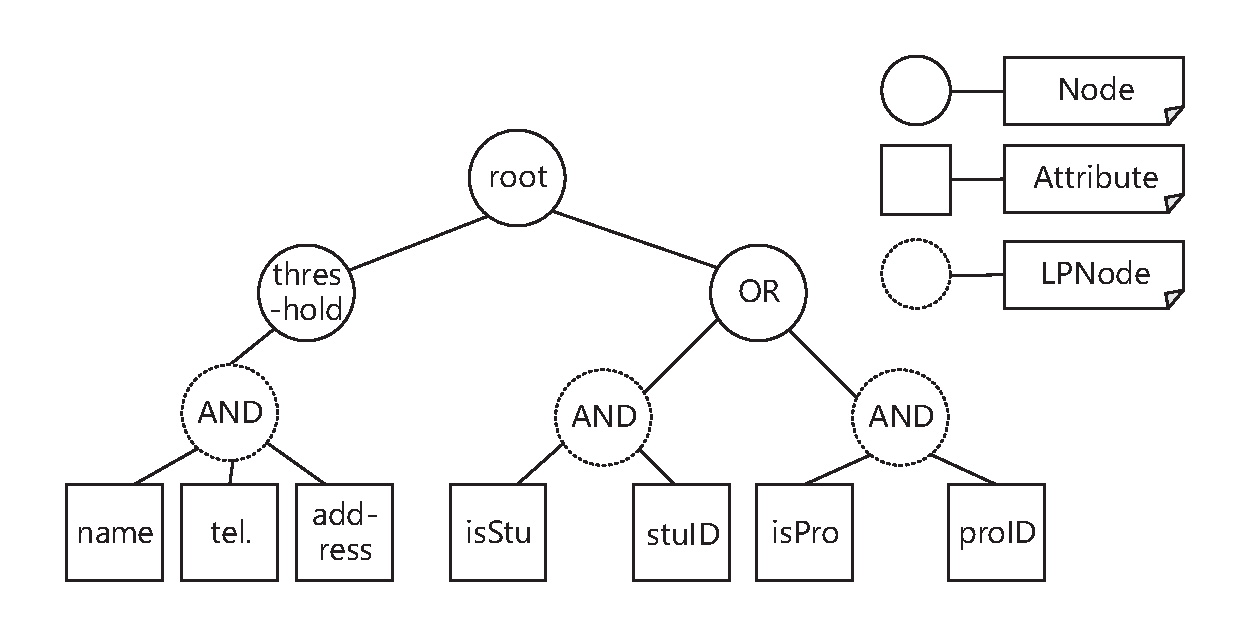
\includegraphics[width=4.3in, keepaspectratio]{figure}
	\caption{Access Tree}
	\label{figure1}
\end{figure}

\subsection{Access Tree}

	To enhance the expression capability of access structure, we utilize tree structure in our scheme. 
	Let $\mathcal{T}$ represents a hierarchical tree. 
	The inner nodes of $\mathcal{T}$ are described the logic relationship of different access policies, including \textit{AND, OR, Threshold}. 
	Besides, the leaf nodes of $\mathcal{T}$ represent attribute marked $a_i=v_{i,t_i}(i \in \mathbb{Z}_n,t_i \in \mathbb{Z}_{n_i})$. 
	For each leaf node, we can always seek its parent node and called it \textit{LPNode} for simplicity. In our tree structure \textit{LPNode} can only express the \textit{AND} relationship.
	Hence, it is obvious that a kind of attribute value can only appear once under each \textit{LPNode}. 
	Here is an access tree example in Figure\ref{figure1}.

\subsection{Our Scheme}
Our scheme is consisted of the following algorithm:
\begin{itemize}
	\item Setup($1^\lambda$): 
		TA runs algorithm $\mathcal{G}(1^\lambda)$ to product four elements including $N=p\cdot q \cdot r,\mathbb{G},\mathbb{G}_T,e$. 
		The subgroups $\mathbb{G}_p,\mathbb{G}_q,\mathbb{G}_r$ are from group $\mathbb{G}$. 
		Note that, the subgroup $\mathbb{G}_p$ is used to subsequent steps. 
		Considering security of the whole scheme, the subgroup $\mathbb{G}_r$ is used to generate random parameters. 
		The subgroup $\mathbb{G}_q$ is mainly used to security analysis. 
		And $g_p,g_q,g_r$ are the generators of three subgroups $\mathbb{G}_p,\mathbb{G}_q,\mathbb{G}_r$. $\mathbb{U}=\{a_1,a_2,\dots,a_n\}$ expresses all the attributes in the whole system. 
		For each attribute, TA randomly chooses $a_{i,t_i} \in \mathbb{Z}_N, R_{i,t_i} \in \mathbb{Z}_n$ and calculates $A_{i,t_i}=g_{p}^{a_{i,t_i}}R_{i,t_i}$. 
		In addition, TA generates three more parameters $\omega, \bar{\omega} \in \mathbb{Z}_N/0$ and $R_0 \in \mathbb{G}_r$. 
		Two more parameters $u,v \in \mathbb{G}_p$ and a key derivation function \textbf{KDF} with output length $\ell$ are chosen by TA.
		Last, TA computes $A_0=g_pR_0,Y=e(g_p,g_p)^{\omega},\bar{Y}=e(g_p,g_p)^{\bar{\omega}}$. 
		The public key $PK$ and master secret key $MSK$ are defined as formula(\ref{PK}) and (\ref{MSK}):  
		
		\begin{equation}\label{PK}
			PK=\left( A_0,g_r,\{A_{i,t_i}\}_{1\leq t_i \leq n_i, 1 \leq i \leq n},Y,\bar{Y}, u, v, \textbf{KDF}, \ell \right)
		\end{equation}
		\begin{equation}\label{MSK}
			MSK=\langle g_p,\{a_{i,t_i}\}_{1\leq t_i \leq n_i, 1 \leq i \leq n},\omega,\bar{\omega}\rangle
		\end{equation}


	\item KeyGen(MSK,PK,L): For $\forall i \in \mathbb{Z}_k$, the DO randomly selects $d_i \in \mathbb{Z}_N$. Therefore, the $SK_L$ is like the format of formula(\ref{SK}):
	\begin{equation}\label{SK}
		SK_L=\langle D_0=g_p^{\omega - \sum_{i=1}^{k}d_i}, \bar{D}_0=g_p^{\bar{\omega} - \sum_{i=1}^{k}d_i}, \{D_j=g_p^{\frac{d_i}{a_{i,t_i}}}\}_{1 \leq i \leq k } \rangle
	\end{equation}


	\item Encrypt(PK,m,T): 
		\begin{itemize}
			\item [a).]	DO selects random values $R_0' \in \mathbb{G}_r$ and $s \in \mathbb{Z}_N$ to encrypt the message $m \in \mathbb{G}$ as follows:
						\begin{equation}
							C_0 = A_0^sR'_0, \ \tilde{C} = mY^s
						\end{equation}

			\item [b).] DO sets a session key $\textbf{DK}=e(g_p,g_p)^{\omega s}$, and computes $\textbf{KDF}(\textbf{DK}, \ell) = VKEY \parallel \eta $ where $\eta$ is a random number and $VKEY$ is used to verify.
						Then $\widehat{C}=u^{H(VKEY)}v^{H(\eta)}$.
						
			\item [c).] Let secret $s$ be assigned in access tree and the root node of $\mathcal{T}$ is set to be $s$. 
						All child nodes except for leaf nodes are marked un-assigned status and root node is assigned status.
						Then, for each unassigned node, do the following operations recursively:
						\begin{itemize}
							\item [$\bullet$] If the node logic operator is \textit{AND}, the first $u-1$ child nodes are set to $s_i$ where $s_i$ is randomly generated in $\mathbb{Z}_N$, and the last child node is set to $s_u=s-\sum_{i=1}^{u-1}s_i$;
							\item [$\bullet$] If the node logic operator is \textit{OR},  the child nodes of this node are set $s$;	
							\item [$\bullet$] If the node logic operator is \textit{Threshold} with the threshold value $h$, it will arbitrarily generate a polynomial $f$ that satisfies $f(0)=s$ and the degree of polynomial is $h-1$. For the i-th node, the value is assigned $f(i)$. 
						\end{itemize}
			\item [d).] Suppose that a \textit{LPNode} in access tree has a shared secret $s_\alpha$. 
						Then calculate a ciphertext component for each attribute in system according to formula(\ref{CT}), where $s_{i,t_i} \in \mathbb{Z}_N$ is a random value and $R'_{i,t_i}$ is also a random parameter produced from $\mathbb{G}_r$. 
						Therefore, the ciphertext of \textit{LPNode} is like formula(\ref{Ca}):
			\begin{equation}\label{CT}
				C_{i,t_i}=
				\begin{cases}
				A_{i,t_i}^{s_{i,t_i}}R'_{i,t_i}, &\text{$L_i \in L_\alpha \ and \ v_{i,t_i} \notin L_\alpha$}\\
				A_{i,t_i}^{s_{\alpha}}R'_{i,t_i}, &\text{otherwise}
				\end{cases}
			\end{equation}
			\begin{equation}\label{Ca}
				C_\alpha = \langle H_\alpha=\bar{Y}^{s_\alpha}, \bar{C}_\alpha=A_0^{s_\alpha}R_\alpha, \{C_{i,t_i}\}_{i \leq t_i \leq n_i, 1 \leq i \leq n} \rangle
			\end{equation}
			where $R_\alpha \in \mathbb{G}_r$. Ultimately, output the final ciphertext:
			\begin{equation}
				CT=\langle \tilde{C},C_0,\{C_\alpha\}_{\forall \alpha \ in \ T}, \widehat{C} \rangle
			\end{equation}
		\end{itemize}
	
	



	\item GenToken(CT,SK): DO selects a random factor $z \in \mathbb{Z}_N$ and does the following operations: $D_i^*=D_i^z,\bar{D}_0^*=\bar{D}_0^z,D_0^*=D_0^z,H_\alpha^*=H_\alpha^z$. 
	Finally, the DO output the TK as the formula(\ref{TK}) and CT to outsourced server by security channel.
	\begin{equation}\label{TK}\\
		TK=\langle D_i^*,\bar{D}_0^*,H^*_\alpha  \rangle
	\end{equation}
	\item PreDecrypt(CT,TK,PK): 
	In this process, outsourced server runs the following defined functions. 
	If the node is a \textit{LPNode}, it will execute \textit{PreDecNode($\alpha$)}. 
	Similarly, if the node is a normal node, it will execute \textit{PreDecNode($\beta$)} where $u$ is the number of child of node $\beta$ and $h$ is the threshold value of node $\beta$.
	\begin{equation}\label{PreDecNodeA}
		PreDecNode(\alpha)=\prod_{i=1}^{k}e(C_{i,t_i},D_i^*)
	\end{equation}
	PreDecNode($\beta$)
	\begin{equation}\label{PreDecNodeB}
		=
		\begin{cases}
		% \prod_{i=1}^{h}PreDecNode(Child(\beta,i))^{\prod_{j=1,j\neq i}^{h}\frac{i}{j-i}}, &Option(\beta)=Threshold\\
		\prod_{i=1}^{h}PreDecNode(Child(\beta,i))^{\Delta_{i,\beta}(0)}, &Option(\beta)=Threshold\\
		\prod_{i=1}^{u}PreDecNode(Child(\beta,i)), &Option(\beta)=AND\\
		PreDecNode(Child(\beta,i)), &Option(\beta)=OR
		\end{cases}
	\end{equation}
	\item Testing: The outsourced server calculates $\theta_\alpha=\frac{H_\alpha^*}{e(\bar{C}_\alpha,\bar{D_0}^*)PreDecNode(\alpha)}$. 
	If the \textit{LPNode} satisfies the attributes represented by each leaf node under it, then it can obtain $PreDecNode(\alpha)=e(g_p,g_p)^{zds_\alpha}$. Further, the outsourced server performs the following calculations:
	\begin{equation}
		\begin{split}
			\theta_\alpha &=\frac{H_\alpha^*}{e(\bar{C}_\alpha,\bar{D_0}^*)PreDecNode(\alpha)}\\
						  &=\frac{\bar{Y}^{zs_\alpha}}{e(A_0^{s_\alpha}R_\alpha,g_p^{z(\bar{\omega}-d)})e(g_p,g_p)^{zds_\alpha}}\\
						%   &=\frac{e(g_p,g_p)^{\bar{\omega}zs_\alpha}}{e(g_p^{s_\alpha},g_p^{z(\bar{\omega}-d)})e(g_p,g_p)^{zds_\alpha}}\\
						%   &=\frac{e(g_p,g_p)^{\bar{\omega}zs_\alpha}}{e(g_p^{s_\alpha},g_p^{z(\bar{\omega}-d)})	e(g_p,g_p)^{zds_\alpha}}\\
						  &=\frac{e(g_p,g_p)^{\bar{\omega}zs_\alpha}}{e(g_p,g_p)^{zs_\alpha (\bar{\omega}-d)} e(g_p,g_p)^{zds_\alpha}}\\
						  &=1
		\end{split}
	\end{equation}
Evidently $\theta_\alpha$ will be a random value, if the \textit{LPNode} cannot satisfy attributes. 
When $\theta_\alpha$ is a random value, it indicates this \textit{LPNode} is an error node. 
Hence, there is no necessary to participate in the subsequent decryption phase. 
The next description operation is completed by executing formula(\ref{CT2}) when $\theta_\alpha=1$:
\begin{equation}\label{CT2}
	\begin{split}
		X   &=\frac{1}{e(C_0,D_0^*)PreDecNode(root(T))}\\
			&=\frac{1}{e(g_p^sR_0^sR'_0,g_p^{z(\omega-d)})e(g_p,g_p)^{dsz}}\\
			% &=\frac{1}{e(g_p^s,g_p^{z(\omega-d)})e(g_p,g_p)^{dsz}}\\
			&=\frac{1}{e(g_p,g_p)^{sz(\omega -d)}e(g_p,g_p)^{dsz}}\\
			&=\frac{1}{e(g_p,g_p)^{sz\omega}}
	\end{split}
\end{equation}
At last, outsourced server sets $T_1 = \widehat{C}$ and transfers $CT'=\left( T_1, X \right)$ to DataUser.
	\item Decrypt(CT',SK,CT): DataUser receives $CT'$ sent by outsourced server and use $SK$ to decrypt ciphertext. The decryption process is described as formula(\ref{Decrypt}):
	\begin{equation}\label{Decrypt}
		\begin{split}
			\frac{\tilde{C}}{(X)^\frac{1}{z}} &= \frac{mY^s}{e(g_p.g_p)^{s\omega}} 
												= \frac{me(g_p.g_p)^{s\omega}}{e(g_p.g_p)^{s\omega}} 
												= m
		\end{split}
	\end{equation}

	\item Verify(CT,CT'): DataUser verifies the correctness of result generated from outsourced server.
		  The detail procedures are as followings: 
		\begin{itemize}
			\item[a).] If $T_1=\widehat{C}$ holds, let $\textbf{DF}=X^{-\frac{1}{z}}=e(g_p,g_p)^{s \omega}$ and $\textbf{KDF}(\textbf{DK},\ell)=VKEY \parallel \eta$; otherwise, output the terminator $\perp$;
			\item[b).] If $u^{H(VKEY)}v^{H(\eta)}=\widehat{C}$ holds, it denotes the testing results and outsourced decryption are proper, furthermore, DataUser can calculate a right message $m$; otherwise, output the terminator $\perp$; 
		\end{itemize}
\end{itemize}

 
\section{Security Proof}\label{section4}
In this section, we will give a proof of security of our scheme. The idea of Lai et.al inspires our thinking and based on dual encryption system invented by Waters et.al we completed our proof. Above all, for convenience, we denote the corresponding definitions used in Water's paper. Both ciphertext and private keys can take on one of two indistinguishable forms the \textit{normal} or the \textit{semi-functional} in dual system encryption system. A \textit{normal} private key or ciphertext are generated from key generation or encryption algorithm. As for semi-functional private key, it can decrypt all normally generated ciphertext. However, decryption will fail if one try to decrypt a semi-functional ciphertext with a semi-functional privacy key. Similarly, semi-functional ciphertext can be decrypted only by normal private key. Note that the semi-functional ciphertext and semi-functional private keys are used in our proof process, and you can't search for them in the actual system.\\
The security of our scheme depends on three hypotheses which are mentioned in section \ref{Complexity_Assumptions} and we utilize hybrid argumentation techniques to prove the security of the scheme with the indistinguishability of a series of games. The followings displayed are the components of our proof procedure.
\begin{itemize}
	\item Normal ciphertext: The normal ciphertext is like: 
	\begin{equation}
		\langle \tilde{C'},C'_0,\{(C'_{i,t_i})_{1 \leq t_i \leq n_i, 1 \leq i \leq n}\}  \rangle
	\end{equation}
	\item Semi-functional ciphertext: Select a random number $x_0 \in \mathbb{Z}_N/0$ and in each \textit{LINode}, for $\forall t_i(i \in \mathbb{Z}_n/0,t_i \in \mathbb{Z}_{n_i}/0)$, randomly generates $x_{i, t_i} \in \mathbb{Z}_N/0$, then, the semi-functional ciphertext is: 
	\begin{equation}
		\langle \tilde{C}=\tilde{C'},C_0=C'_0g_q^{x_0},\{C_{i,t_i}=C'_{i,t_i}g_q^{x_{i,t_i}}\}_{1 \leq t_i \leq n_i, 1 \leq i \leq n} \rangle
	\end{equation}	
\end{itemize}
\begin{itemize}
	\item $Game_{real}$: The real game is composed of real private key and ciphertext;
	\item $Game_0$: The query private key is normal but challenge ciphertext is semi-functional in $Game_0$;
	\item $Game_{1,k}$: It denotes the challenge ciphertext is semi-functional. The private key of the first queries is semi-functional and the remains are normal.
	\item $Game_{final}$: The private key of all queries is semi-functional. The challenge ciphertext is a semi-functional ciphertext generated by encrypting a random message.
\end{itemize}
\newtheorem{myLemma}{Lemma}
\begin{myLemma}
	Suppose there exist a probabilistic polynomial time algorithm $\mathcal{A}$ that can win $Gmae_{real},Game_0$ with advantage $Adv^{Game_{real}}_{\mathcal{A}}-Adv^{Game_0}_{\mathcal{A}}=\varepsilon$. Then we can build a PPT algorithm $\mathcal{C}$ to break Assumption\ref{myAssumption1} with advantage $\varepsilon$.
\end{myLemma}
\begin{proof}
	Given the distribution in Assumption\ref{myAssumption1}, $D=\{\mathbb{G},g_p,g_r\}$.
	\begin{itemize}
		\item Setup: This phase is the same as Setup algorithm in section 3.3.
		\item Phase1: Adversary can answer private key of any attribute set.
		\item Challenge: Adversary selects two messages $m_0,m_1$ with the same length and two access structures $T_0,T_1$. Note that any query cannot satisfy access structures $T_0,T_1$.	Then adversary transfers them to challenger. After the challenger receives the parameters from adversary, challenger flips a coin $b\in\{0,1\}$ and encrypts the received message to $m_b$ by using a access structure $T_b$. Afterwards, challenger randomly selects some necessary parameters, $s\in \mathbb{Z}_N, R'_0 \in \mathbb{G}_r$ and generates $\tilde{C}^*=m_be(g_p,X)^{\omega s}, C_0^*=X^sR'_0$ which are components of ciphertext. When $((L_i \in L_\alpha)\wedge(v_{i,t_i} \notin L_\alpha))$, challenger obtains the random value $s_{i,t_i} \in \mathbb{Z}_N \  and \  s_{i,t_i} \neq s_\alpha$, set $C^*_{i,t_i}=X^{a_{i,t_i}\cdot s_{i,t_i}}R'_{i,t_i}$, otherwise, let $C^*_{i,t_i}=X^{a_{i,t_i}\cdot s_{\alpha}}R'_{i,t_i}$. Finally, challenger send the completed ciphertext $\langle \tilde{C}^*, C_0^*, \{\{C^*_{i,t_i}\}_{1 \leq i \leq n, 1 \leq t_i \leq n_i}\}_{\forall \alpha}\rangle$ to $\mathcal{A}$.
		\item Phase2: It is the same as Phase1.
		\item Guess: Adversary outputs a guess $d'$ to challenger.
	\end{itemize}
	Apparently, if $X \in \mathbb{G}_p$ the answer ciphertext $c*$ must be normal ciphertext. Similarly, if $X \in \mathbb{G}_{pq}$, the answer ciphertext $c*$ have semi-function. Therefore, under the assumption that $\mathcal{A}$ have a non-negligible advantage $Adv_{\mathcal{A}}^{Game_{real}}-Adv_{\mathcal{A}}^{Game_0}=\varepsilon$, then challenger also can distinguish elements of $\mathbb{G}_p$ or $\mathbb{G}_{pq}$ with indistinguishable advantage.
\end{proof}

\begin{myLemma}
	If there exist a algorithm $\mathcal{A}$ that can distinguish between $Game_{real}$ and $Game_{0}$ with advantage $Adv_{\mathcal{A}}^{Game_{real}}-Adv_{\mathcal{A}}^{Game_0}=\varepsilon$, then a algorithm $\mathcal{C}$ that can break Assumption\ref{myAssumption2} with identical advantage $\varepsilon$ in probabilistic polynomial time is constructed.	
\end{myLemma}
\begin{proof}
	Given the same conditions as Assumption\ref{myAssumption2}
	\begin{itemize}
		\item Setup: the similar step as in Lemma1.
		\item Challenge: In this phase, $\mathcal{A}$ sends the followings that consists of $m_0,m_1$ with the same bit-length and two access structure $T_0,T_1$(note that any attribute set can not satisfy them) to challenger. Subsequently, challenger selects a random value $b \in {0,1}$ and use the access structure $T_b$ to encrypt message to generate new ciphertext $m_b$. Then challenger arbitrarily chooses $s \in \mathbb{Z}_N,R'_0 \in \mathbb{Z}_r$ and produces the semi-functional ciphertext by the corresponding parameters in $MSK$ and assumption conditions $\tilde{C}^*=m_be(g_p,X_1X_2)^{\omega s}, C_0 = (X_1,X_2)^sR'_0$. Finally, when $((L_i \in L_\alpha)\wedge(v_{i,t_i} \notin L_\alpha))$, let $C^{*}_{i,t_i}=(X_1X_2)^{a_{i,t_i}s_{i,t_i}}R'_{i,t_i}$ where $s_{i,t_i}$ is a random value and $s_{i,t_i} \in \mathbb{Z}_N \ and \ s_{i,t_i} \neq s_\alpha$, otherwise, let $C^{*}_{i,t_i}=(X_1X_2)^{a_{i,t_i}s_\alpha}R'_{i,t_i}$. Hence, the ciphertext $\langle \tilde{C}^*, C_0^*, \{\{C^*_{i,t_i}\}_{1 \leq i \leq n, 1 \leq t_i \leq n_i}\}_{\forall \alpha}\rangle$ is transmit to $\mathcal{A}$. 
		\item Phase1 and Phase2: Considering the $i-th$ query of $\mathcal{A}$, obviously, the private key query is divided the following three sections: 
		\begin{itemize}
			\item[$\bullet$] Case1: When $i>k$, challenger can correctly calculate normal private key using $MSK$ and attribute sets from the query of $\mathcal{A}$, then challenger sends the normal private key to $\mathcal{A}$.
			\item[$\bullet$] Case2: When $i<k$, according to the above definition of $Game_{1,k}$, the first $k-1$ private key of $Game_{1,k-1}$ and $Game_{1,k}$ is semi-functional. Therefore, challenger calculates to the semi-functional key and sends it to $\mathcal{A}$.
			\item[$\bullet$] Case3: When $i=k$, for $\forall i \in \mathbb{Z}_k$, challenger randomly chooses $d_i \in \mathbb{Z}_N$ and generates private key $D'_0=X^{\omega-d}, D'_i=X^{\frac{d_i}{a_{i,t_i}}}$ where $d_i \in \mathbb{Z}_N$,$d_i$ is a random value and sets $d=\sum_{i=1}^{k}d_i$. 
		\end{itemize}
		\item Guess: Adversary outputs a guess $d'$ to challenger.
	\end{itemize}
	One situation is that if $X \in \mathbb{G}_p$, let $X=\mathbb{G}_p$, hence, the generated key is normal private key, further, the game is $Game_{1,k-1}$. The other is that $X=g_pg_q^{\frac{y_0}{\omega -d}},X \in \mathbb{G}_{pq}$, moreover, the generated private key is semi-functional key and the game is $Game_{1,k}$. Therefore, considering the above two situation, if $\mathcal{A}$ has a non-negligible advantage $Ada_{\mathcal{A}}^{Game_{1,k-1}}-Ada_{\mathcal{A}}^{Game_{1,k}}=\varepsilon$, then challenger also has a non-negligible advantage to distinguish the elements between $\mathbb{G}_{pq}$ and $\mathbb{G}_p$.
\end{proof}

\begin{myLemma}
	If there exist a probabilistic polynomial time algorithm $\mathcal{A}$ that has the advantage $Adv_{\mathcal{A}}^{Game_{1,u}}-Adv_{\mathcal{A}}^{Game_{final}}=\varepsilon$, then a probabilistic polynomial time algorithm $\mathcal{C}$ that is able to break Assumption\ref{myAssumption3} with the advantage $\varepsilon$ can be built.
\end{myLemma}
\begin{proof}
	Given the distributions in Assumption\ref{myAssumption3}, $D=(\mathbb{G},g_p,g_p^{\omega}X_2,g_p^{s}Y_2,Z_1Z_2g_r)$.
	\begin{itemize}
		\item Setup: Repeat the step in Lemma1.
		\item Phase1 and Phase 2: In $Game_{1,u}$ and $Game_{final}$, the generated private keys are semi-functional. The challenger produces semi-functional private keys $D'_0=g_p^{\omega}X_2(Z_1Z_2)^{-d},D'_i=(Z_1Z_2)^{\frac{d_i}{a_{i,t_i}}}$ based on queried attributes sets by $\mathcal{A}$ where $i \in \mathbb{Z}_k, d_i \in \mathbb{Z}_N$ are random values and set $d = \sum_{i=1}^{k}d_i$. 
		\item Challenge: $\mathcal{A}$ arbitrarily selects two messages $m_0,m_1$ with the same length and two access structures $T_0,T_1$ that cannot be satisfied by any attribute set. Then $\mathcal{A}$ sends them to challenger. Challenger use access structure $T_b$ to encrypt the message to generate $m_b$ or a random value $r$. Subsequently, challenger arbitrarily chooses $s$ and do the following operations to produce component of ciphertext. $\tilde{C}^*=m_bT, C_0^*=g_p^sY_2R'_0$. The remain ciphertext components are obtained by the following calculations. When $(L_i \in L_\alpha)\wedge(v_{i,t_i} \notin L_\alpha)$, let $C^*_{i,t_i}=g_p^{a_{i,t_i}s_{i,t_i}}R'_{i,t_i}$ where $s_{i,t_i} \in \mathbb{Z}_N \ and \  s_{i,t_i} \neq s_\alpha$, otherwise, $C^*_{i,t_i}=g_p^{a_{i,t_i}s_{\alpha}}R'_{i,t_i}$. Lastly, the whole ciphertext $\langle \tilde{C}^*,C_0^*,C^{*}_{i,t_i}\rangle$ is dispatched to $\mathcal{A}$.
		\item Guess: Challenger outputs a guess marked $d'$ of $d$.  
	\end{itemize}
	When $T=e(g_p,g_p)^{\omega s}$, encrypted message $m_b$ is a semi-functional ciphertext, otherwise, let $T=e(g_p,g_p)^{\omega s - x_0}$, the generated semi-functional ciphertext belongs to the random message $m_be(g_p,g_p)^{\omega s-x_0}$. Therefore, If $\mathcal{A}$ has a non-negligible advantage $Adv_{\mathcal{A}}^{Game_{1,u}} - Adv_{\mathcal{A}}^{Game_{final}}=\varepsilon$, then challenger can also distinguish a random element between $e(g_p,g_p)^{\omega s}$ and $\mathbb{G}_T$ with non-negligible advantage. 
\end{proof}
\begin{myDefinition}
	Assume that Assumption\ref{myAssumption1},Assumption\ref{myAssumption2} and Assumption\ref{myAssumption3} hold, then the scheme described in this paper is secure.
\end{myDefinition}
\begin{proof}
	If Assumption\ref{myAssumption1},Assumption\ref{myAssumption2} and Assumption\ref{myAssumption3} hold, $Game_{real}$ and $Game_{finla}$ are indistinguishable, furthermore, $\mathcal{A}$ has a negligible advantage $Adv_{\mathcal{A}}^{Game_{final}}$ in $Game_{final}$, hence, $\mathcal{A}$ have a negligible advantage $Adv_{\mathcal{A}}^{Game_{real}}$ in $Game_{real}$. So, our scheme satisfies security under Chosen Ciphertext Attack(CCA). 
\end{proof}
\section{Performance Analysis}\label{section5}
In this section, we reveal the performance of our scheme and it is divided into two sections theoretical analysis and experimental simulation. 
In the former, we mainly adopt mathematical methods to analyze the efficiency of our scheme and the length of ciphertext, and compare it with other schemes. 
In order to verify the correctness of the theoretical analysis scheme, we conducted a simulation experiment in the latter. 
\subsection{Theoretical Analysis}

Table\ref{propertyTable} indicates the properties between our scheme and other related scheme. 
$\checkmark$ means the scheme satisfies this property, conversely, $\times$ shows the schemes can not match this property. 
From Table\ref{propertyTable}, we can get the conclusion that compared with other schemes, our scheme not only has strong expressive ability, but also has more comprehensive features to improve efficient.  

Firstly, let us present the notations appearing in the following. $N$ expresses the number of attributes in the whole system. $T_{\mathbb{G}},T_{\mathbb{G}_T}$ indicate the cost time of operations of group $\mathbb{G}$ and group $\mathbb{G}_T$. Note that the operations only include exponentiation for convenience. $|*|$ is the bit-length of $*$. 
% table1
\begin{table}[h] 
	\caption{PROPERTY COMPARISON TABLE}
	\resizebox{\textwidth}{13mm}
	{
	% \begin{tabular}{p{3cm}|p{5cm}|p{5cm}} %设置了每一列的宽度,强制转换。
	\begin{tabular}{cccccc}
	\toprule[1.5pt]
	\textbf{Scheme} & \textbf{Access Structure} & \textbf{Hidden Policy} & \textbf{Testing} & \textbf{Outsourcing} & \textbf{Security Model} \\ %用&来分隔单元格的内容 \\表示进入下一行
	\midrule %画一个横线,下面的就都是一样了,这里一共有4行内容
	Nishide & AND-gates & \checkmark & $\times$ & $\times$ & selectively-CCA \\
	Lai     & AND-gates & \checkmark & $\times$ & $\times$  & adaptively-CCA \\
	Luan    & Tree & $\times$ & $\times$ & $\times$ & selectively-CPA \\
	Li		& AND-gates & \checkmark & \checkmark & $\times$ &  selective-CPA\\
	Xu		& Tree		& \checkmark & $\times$   & $\times$ & selectively-CPA\\	
	Ours    & Tree & \checkmark & \checkmark & \checkmark & adaptively-CCA \\
	\bottomrule[1.5pt]
	\end{tabular}
	}
	\label{propertyTable}
\end{table}

\subsection{Experimental Simulation}


\end{document}








